\documentclass[conference]{IEEEtran}
% For A4 paper instead of US Letter, use: \documentclass[conference,a4paper]{IEEEtran}
\IEEEoverridecommandlockouts
\usepackage{cite}
\usepackage{amsmath,amssymb,amsfonts}
\usepackage{graphicx}
\usepackage{textcomp}
\usepackage{booktabs}
\usepackage{url}
\usepackage{xcolor}


\begin{document}

\title{Choosing Proxy Languages for Speech Recognition of Unwritten Indian Dialects Using Correction Effort}

\author{
\IEEEauthorblockN{Laksh Yadav, Mikul Swamy, Mohamad Aashim, Mohamed Ali and Priyanka K R}
\IEEEauthorblockA{\textit{Department of Computer Science and Engineering} \\
\textit{RV Institute of Technology and Management}\\
Bengaluru, India \\
\{lakshyadav1212, mikulnswamy07, mohamad.aashim11, mohamedali04123\}@gmail.com, priyankakr.rvitm@rvei.edu.in}
}

\maketitle

\begin{abstract}
Most of India's spoken varieties have little or no written text and are not supported by speech recognition. Multilingual models such as Whisper can transcribe an unsupported dialect only as one of the languages they know, and the best choice of this \emph{proxy language} is not obvious: Tulu, for example, is written in Kannada script but is lexically distinct from Kannada. We present SwaraVeda, a deployed, consent-first community archive in which members record speech in the browser (also offline), an assistant named Vani drafts a time-aligned transcript with Whisper large-v3, native speakers correct every passage while listening, and verifiers approve it. Because the archive keeps both the machine draft and the human correction of every passage, the edit distance between them is available at no extra annotation cost. We propose using this correction effort as a signal to rank candidate proxy languages per dialect and to update the choice as verified data accumulates, and implement this selection in the archive. On 100 utterances of Odia, an Indian language that Whisper does not support, from the FLEURS benchmark, correction effort selects Hindi rather than the related Bengali and Assamese and lowers the character error rate from 44.6\% with automatic language identification to 37.7\%. The archive catalogues 139 dialects with their script, region, ISO 639-3 code and a proxy-language hint, separates consent for public listening from consent for AI training, and exports verified passages as a training dataset for future dialect-specific models.
\end{abstract}

\begin{IEEEkeywords}
endangered languages, low-resource speech recognition, Whisper, human-in-the-loop, language documentation, proxy language, consent, Indian dialects
\end{IEEEkeywords}

\section{Introduction}
In the 2011 Census of India, people named 19,569 different mother tongues; after linguistic scrutiny the Census counted 1,369 of them and classified these under 121 languages \cite{census2011}. Many of the remaining varieties are spoken mainly by small and ageing communities and are classified as vulnerable or endangered \cite{unesco2010}. Their songs, rituals and everyday speech, such as the Tulu \emph{paddanas} of coastal Karnataka, survive only orally. When the last fluent speakers are gone, this knowledge is lost.

Speech technology could help preserve these varieties, but it needs transcribed audio, which these dialects do not have. Large multilingual models such as Whisper \cite{radford2023} and MMS \cite{pratap2024} cover major Indian languages but not dialects such as Tulu, Toda, Kodava or Beary; only recent models fine-tuned on new corpora such as Vaani begin to include a few of them \cite{sravaani}. Manual transcription by linguists is slow, so field recordings often remain unused.

A practical workaround is to transcribe an unsupported dialect \emph{as if} it were a related, supported language, the \emph{proxy language}, and let native speakers correct the result. The quality of the first draft, and therefore the correction effort, depends on that choice. The right proxy is not always the language that shares the script: Tulu uses Kannada script but is a separate South Dravidian language, and Beary is written in Kannada or Malayalam script while being closest to Malayalam.

This paper makes the following contributions:
\begin{itemize}
\item \textbf{SwaraVeda}, a deployed web archive for endangered Indian dialects that combines in-browser and offline recording, per-recording dual consent, AI drafting, community correction and verification, and search by words and by meaning (Section~\ref{sec:system}).
\item \textbf{Correction effort as a signal}: a method that uses the edit distance between Whisper's draft and the verified human correction to rank and update the proxy language of each dialect, without any annotation beyond the community's normal work (Section~\ref{sec:method}).
\item A catalogue of \textbf{139 Indian dialects} with script, region, ISO 639-3 code and a proxy-language hint, and a \textbf{consent-scoped dataset export} that pairs every machine draft with its correction (Sections~\ref{sec:system} and \ref{sec:results}).
\item An implementation of this selection inside the deployed archive, per-dialect pilot data from it, and an evaluation on Odia from the FLEURS benchmark in which the selected proxy lowers the character error rate by 6.9 points relative to automatic language identification (Sections~\ref{sec:system}, \ref{sec:setup} and \ref{sec:results}).
\end{itemize}

\section{Related Work}
\subsection{Tools for Language Documentation}
Aikuma \cite{bird2014} introduced a mobile app for recording, respeaking and translating endangered-language speech, and LIG-Aikuma \cite{blachon2016} extended it for parallel speech collection in the field. ELPIS \cite{foley2018} lets documentary linguists train speech recognisers on their own transcribed recordings using the Kaldi toolkit \cite{povey2011}. These tools assume that a linguist transcribes or curates the data; they do not use a large pretrained model to produce the first draft, and they do not choose a proxy language.

\subsection{Crowdsourced Speech Corpora}
Mozilla Common Voice \cite{ardila2020} collects read sentences and validates clips by community votes. Karya \cite{abraham2020} crowdsources speech data for Indian languages from low-income workers, and IndicSUPERB \cite{javed2023} released the Kathbath corpus for 12 Indian languages. Read-speech collection requires written prompts, which unwritten dialects lack, and it does not capture songs, stories or spontaneous conversation.

\subsection{Multilingual and Low-Resource ASR}
Self-supervised models such as wav2vec~2.0 \cite{baevski2020} reduce the labelled data needed for a new language, and IndicWav2Vec \cite{javed2022} pretrains on 40 Indian languages. MMS \cite{pratap2024} scales speech recognition to over 1,100 languages using language-specific adapters, while Whisper \cite{radford2023} is trained with weak supervision on 680,000 hours of audio and outputs timestamps and translations. All still require labelled data or a supported language identifier for each target variety; none tells us which supported language best stands in for an unsupported dialect.

\subsection{Choosing a Stand-in Language}
When fine-tuning is not feasible, the common practice for a language Whisper does not support is to reuse the tag of the closest supported language; Huang \textit{et al.} \cite{huang2025} instead combine the embeddings of several language tags, weighted by Whisper's predicted language probabilities. Dhasmana \textit{et al.} \cite{dhasmana2026} show for 30 Indic varieties of the Vaani corpus that phylogenetic distance only partly explains cross-lingual transfer, and Kumar \textit{et al.} \cite{kumar2022} compare ASR for Awadhi, Bhojpuri, Braj and Magahi against a zero-shot Hindi system. For unwritten tribal languages of Karnataka, Rajkhowa \textit{et al.} \cite{rajkhowa2023} transliterate Lambani and Soliga speech into Kannada script. These works choose or combine languages from linguistic similarity or model probabilities, once and offline.

\subsection{Data Governance}
The CARE principles \cite{carroll2020} argue that data about Indigenous peoples should serve collective benefit and remain under community authority. Many speech-collection efforts record a single consent that covers all uses. SwaraVeda separates consent to \emph{listen} from consent to \emph{train AI} and enforces both in every query and export.

\textbf{Gap.} Prior work selects a stand-in language by linguistic similarity or model probabilities. To the best of our knowledge, based on a search of IEEE Xplore, the ACL Anthology and arXiv in November 2026, no prior system selects it from the correction effort of community post-editing or keeps the choice up to date as verified data grows.

\section{System Design}\label{sec:system}
\subsection{Architecture}
SwaraVeda is a three-tier web application (Fig.~\ref{fig:arch}). A React and TypeScript single-page app runs in the browser; a stateless FastAPI service handles authentication, recordings, review, search and export; PostgreSQL with the pgvector extension and an object store hold the data (Supabase). Speech recognition and translation run through hosted model APIs, so the server needs no GPU.

\begin{figure}[t]
\centerline{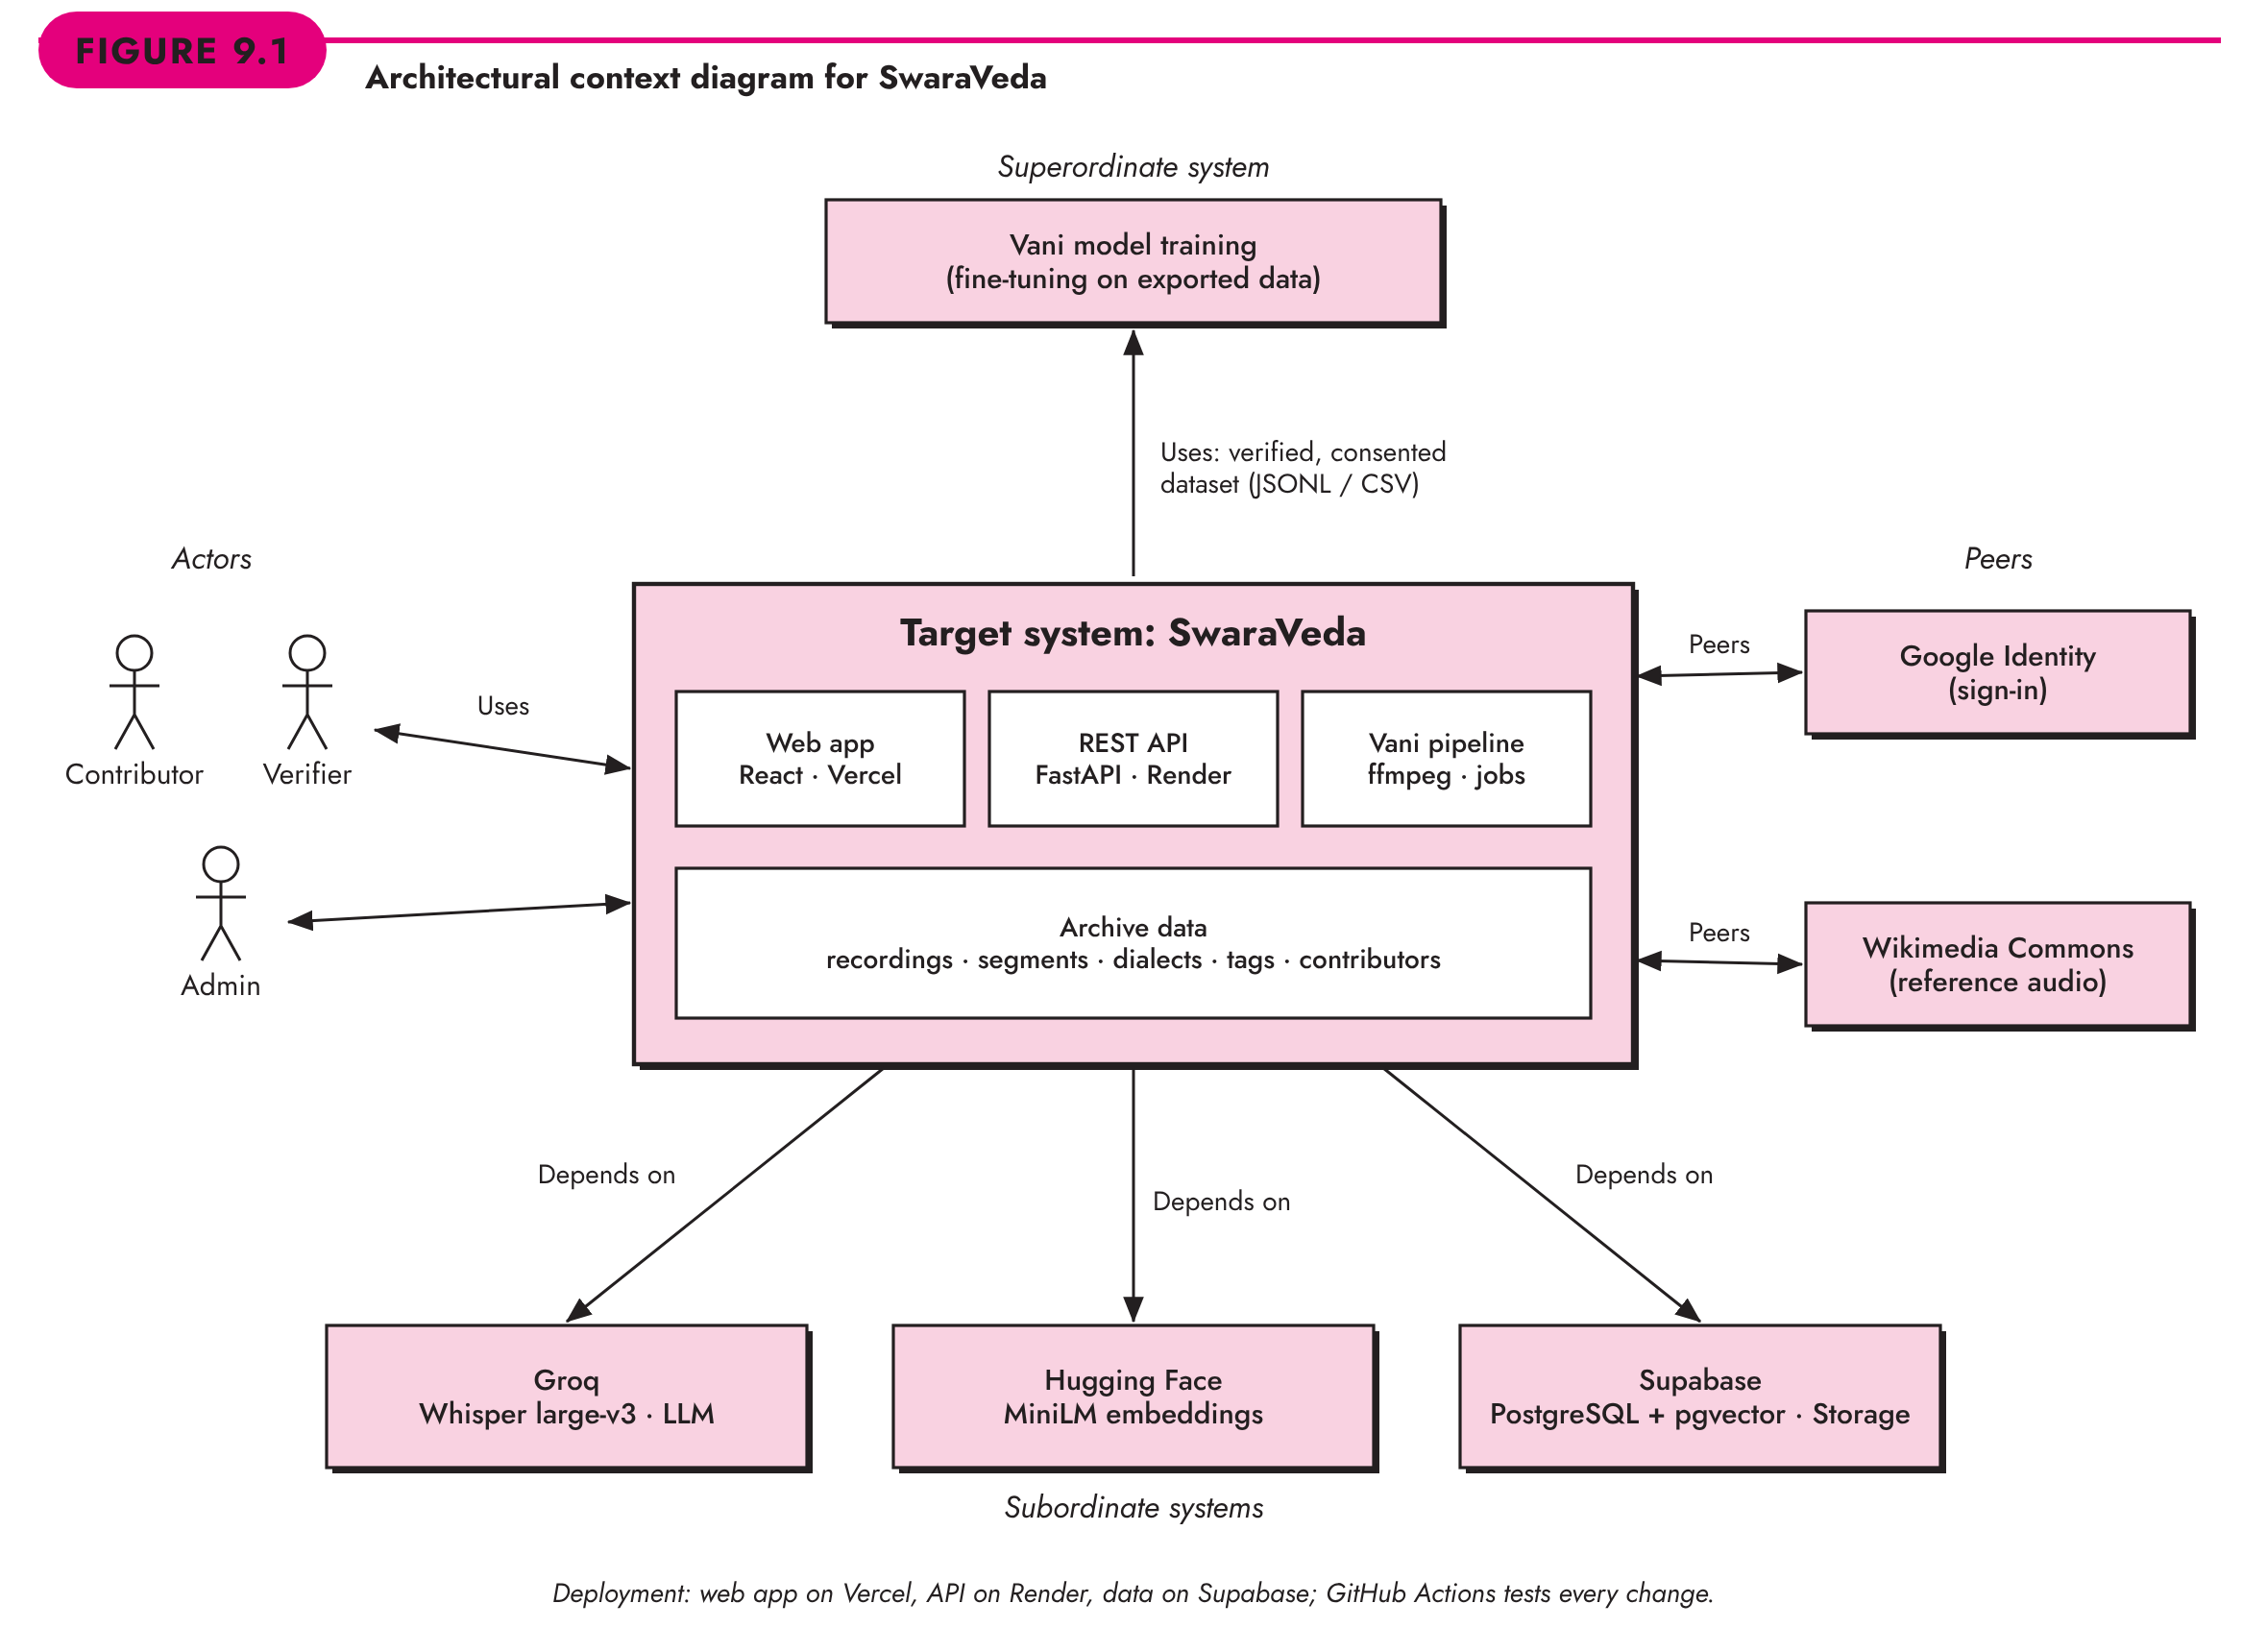
\includegraphics[width=\columnwidth]{fig_architecture.png}}
\caption{Architectural context diagram of SwaraVeda.}
\label{fig:arch}
\end{figure}

\subsection{Capture and Consent}
A three-step form records audio with the browser's MediaRecorder API (or accepts a file) and collects the title, dialect, speaker, genre, place and date. Echo cancellation and noise suppression are disabled, as they distort singing. Two consents are asked separately: whether anyone may listen, and whether the passage may be used to train speech AI. The browser uploads audio directly to storage through a short-lived signed URL. Without a connection, the recording is stored in IndexedDB and uploaded automatically when the browser comes back online; a service worker caches the application so it opens offline.

\subsection{Pre-processing}
Each recording is converted with ffmpeg to 16\,kHz mono, filtered with an 80\,Hz high-pass filter, normalised to $-18$\,LUFS following EBU R\,128 \cite{ebu2020}, and encoded as 32\,kbit/s Opus. In our tests a 2\,MB stereo WAV file became 24\,KB, about 1\% of its size, keeping long recordings under the 25\,MB limit of the recognition API.

\subsection{Transcription with Vani}
Transcription runs as a background job whose progress the client polls. The cleaned audio is sent to Whisper large-v3 \cite{radford2023} with temperature 0 and segment-level timestamps. Each dialect carries a proxy-language code, which is passed as Whisper's language parameter (for example Tulu$\rightarrow$Kannada, Toda$\rightarrow$Tamil, Bhojpuri$\rightarrow$Hindi). The resulting segments, each with start time, end time and draft text, are stored. An LLM then offers an English translation and a Latin-script transliteration of each passage on request.

\subsection{Correction and Verification}
Every segment moves through three states: \emph{needs correction} (machine draft only), \emph{needs verification} (corrected by a native speaker) and \emph{verified} (approved by a verifier). The recording page plays the audio with the current segment highlighted so speakers correct while listening. Verifiers and administrators are assigned by role-based access control; a recording becomes verified when all of its segments are.

\subsection{Search}
Exact-word search uses PostgreSQL full-text search with the language-neutral \emph{simple} configuration and \texttt{ts\_rank} ranking; search by meaning embeds each passage with a multilingual MiniLM sentence encoder \cite{reimers2019,reimers2020} into 384 dimensions and ranks by cosine distance using pgvector \cite{pgvector}. Results play from the segment's start time. Privacy rules apply to every query.

\subsection{Dataset Export}
Verifiers can export, as JSON Lines or CSV, every verified passage whose speaker consented to AI training. Each row holds the audio link, start and end times, the machine draft, the human correction, the transliteration, the translation, the dialect and the licence. This pairing of draft and correction is what the method in Section~\ref{sec:method} relies on.

\subsection{Proxy-Language Selection in the Archive}
The method of Section~\ref{sec:method} is built into the archive. Verifiers see, for every dialect, the character and word error rate between Vani's drafts and the community's corrections, start a comparison of candidate languages that runs as a background job (up to 100 corrected passages, verified ones first or verified ones only, with retries when the speech service rate-limits requests), and switch the dialect's proxy to the best candidate with one click.

\section{Correction Effort as a Proxy-Selection Signal}\label{sec:method}
Let $d$ be a dialect and $L(d)$ a small set of candidate proxy languages, chosen by script and family (for Tulu, \{Kannada, Malayalam\}). For a verified segment $s$ of dialect $d$, let $r_s$ be the human correction and $h_s(\ell)$ the draft produced with proxy $\ell \in L(d)$. With $\mathrm{ED}$ the Levenshtein edit distance \cite{levenshtein1966} over characters, the correction effort of proxy $\ell$ for dialect $d$ is the micro-averaged character error rate
\begin{equation}
C(d,\ell) = \frac{\sum_{s} \mathrm{ED}\big(h_s(\ell),\, r_s\big)}{\sum_{s} |r_s|},
\label{eq:cer}
\end{equation}
computed over the verified segments of $d$. The word error rate $W(d,\ell)$ is defined analogously over words. The archive assigns to each dialect the proxy with the lowest effort:
\begin{equation}
\ell^{*}(d) = \operatorname*{arg\,min}_{\ell \in L(d)} C(d,\ell).
\label{eq:argmin}
\end{equation}

In normal operation each segment is transcribed only with the current proxy, so $C(d,\ell)$ is observed for one $\ell$ only. To compare candidates, the stored audio of a held-out sample of verified segments is re-transcribed with every $\ell \in L(d)$, which costs only API calls, since the human reference $r_s$ already exists. Algorithm~1 summarises the procedure; it is repeated whenever a dialect gains a fixed number $k$ of new verified segments, so the hint improves as the archive grows. Here ``auto'' lets Whisper identify the language itself and serves as the no-hint baseline. The method needs no extra labelling: the references are the corrections the community makes in any case.

\begin{figure}[t]
\hrule\vspace{3pt}
\noindent\textbf{Algorithm 1:} Proxy-language selection from correction effort
\vspace{3pt}\hrule\vspace{4pt}
\small
\noindent\textbf{Input:} dialect $d$, candidates $L(d)$, verified segments $S_d$, sample size $n$\\
\textbf{Output:} proxy $\ell^{*}(d)$
\begin{enumerate}
\setlength{\itemsep}{1pt}
\item $T \leftarrow$ random sample of $\min(n, |S_d|)$ segments of $S_d$
\item \textbf{for each} $\ell \in L(d) \cup \{\text{auto}\}$ \textbf{do}
\item \quad \textbf{for each} $s \in T$: $h_s(\ell) \leftarrow \mathrm{Whisper}(\mathrm{clip}(s), \ell)$
\item \quad $C(d,\ell) \leftarrow$ Eq.~(\ref{eq:cer}) over $T$
\item $\ell^{*}(d) \leftarrow \arg\min_{\ell} C(d,\ell)$; set the hint of $d$ to $\ell^{*}(d)$
\item \textbf{repeat} when $d$ gains $k$ new verified segments
\end{enumerate}
\vspace{2pt}\hrule
\end{figure}

\section{Experimental Setup}\label{sec:setup}
\subsection{Pilot Data in the Archive}
Table~\ref{tab:pilot} lists everything the live archive held when this paper was written: 11 recordings totalling 75\,s from 11 speakers in 8 dialects (two recordings were saved without a dialect), made while testing the system. Of the 12 passages, 5 were corrected and 2 verified, and in every corrected passage the speaker kept Vani's draft unchanged. The table shows how the archive reports data per dialect, but these numbers are far too small to compare proxy languages; recording Tulu, Kodava and Beary in the field is ongoing.

\begin{table}[t]
\caption{Pilot Data in the Live Archive}
\label{tab:pilot}
\centering
\setlength{\tabcolsep}{3pt}
\begin{tabular}{llrrrrr}
\toprule
Dialect & Proxy & Rec. & Speakers & Passages & Corrected & Verified \\
\midrule
Beary & kn & 2 & 2 & 2 & 1 & 1 \\
Birhor & hi & 1 & 1 & 1 & 1 & 0 \\
Havyaka Kannada & kn & 2 & 2 & 3 & 0 & 0 \\
Kundagannada & kn & 1 & 1 & 1 & 1 & 1 \\
Paniya & ml & 1 & 1 & 1 & 0 & 0 \\
Tulu & kn & 1 & 1 & 1 & 1 & 0 \\
Yerukula & te & 1 & 1 & 1 & 1 & 0 \\
No dialect & - & 2 & 2 & 2 & 0 & 0 \\
\midrule
Total & & 11 & 11 & 12 & 5 & 2 \\
\bottomrule
\end{tabular}
\end{table}

\subsection{Benchmark on an Unsupported Indian Language}
To measure the method now, we apply Algorithm~1 to Odia. Odia is a scheduled language of India, but Whisper does not support it: the recognition API rejects its language code. It is therefore in the same position as an unsupported dialect, while the FLEURS benchmark \cite{conneau2023} supplies human-verified transcripts that play the role of the community's verified corrections. We drew a random sample (fixed seed) of 100 utterances from the FLEURS Odia development split (81 distinct sentences, 19.1\,min of read speech). The candidates were Bengali and Assamese, Odia's closest supported relatives in the Eastern Indo-Aryan family; Hindi, the most widely used supported Indo-Aryan language; and automatic identification. Each clip passed through the same pre-processing and Whisper large-v3 call as in the archive (Section~\ref{sec:system}). Whisper writes its draft in the script of the proxy language, so each draft was mapped into Odia script character by character using the parallel layout of the Brahmic Unicode blocks before scoring; a dialect whose proxy uses another script needs the same step. CER and WER follow Eq.~(\ref{eq:cer}) after removing punctuation and normalising Unicode to NFC, and each candidate is also compared with automatic identification utterance by utterance, with a two-sided sign test.

\section{Results}\label{sec:results}
\subsection{Deployed System}
\begin{table}[t]
\caption{Deployed System}
\label{tab:system}
\centering
\begin{tabular}{p{0.36\columnwidth}p{0.54\columnwidth}}
\toprule
Item & Value \\
\midrule
Dialects catalogued & 139, each with script, region, ISO code and proxy hint \\
Audio pre-processing & 2\,MB stereo WAV $\rightarrow$ 24\,KB Opus ($\approx$1\%) \\
Automated backend tests & 127 passing (SQLite and PostgreSQL) \\
Offline capture & IndexedDB queue and service worker \\
Proxy selection & Built in: per-dialect CER/WER and comparison of candidates \\
Deployment & Vercel (web), Render (API), Supabase (data) \\
\bottomrule
\end{tabular}
\end{table}
Table~\ref{tab:system} summarises the deployed system, available at \url{https://swara-veda.vercel.app}. End-to-end browser tests on desktop and phone screen sizes completed the full record, transcribe, correct and verify cycle without errors, and recordings made offline were uploaded and transcribed automatically once the connection returned. Automated tests check the selection logic of Algorithm~1: given drafts produced under each candidate, the archive scores them by Eq.~(\ref{eq:cer}), ranks them, stores the result and names the candidate with the lowest correction effort.

\subsection{Proxy Selection on Odia}
\begin{table}[t]
\caption{Proxy Candidates on FLEURS Odia (100 Utterances)}
\label{tab:fleurs}
\centering
\begin{tabular}{lrrc}
\toprule
Proxy & CER (\%) & WER (\%) & Better / worse than auto \\
\midrule
Bengali (bn) & 44.5 & 91.6 & 16 / 9 \\
Assamese (as) & 60.7 & 105.1 & 19 / 80 \\
\textbf{Hindi (hi)} & \textbf{37.7} & 108.8 & 52 / 42 \\
Automatic & 44.6 & 92.9 & - \\
\bottomrule
\end{tabular}
\end{table}
Table~\ref{tab:fleurs} gives the results. Hindi had the lowest correction effort, a CER of 37.7\% against 44.6\% with automatic identification: a reduction of 6.9 points, with a 95\% bootstrap confidence interval of 4.2 to 9.6 points over utterances. Algorithm~1 therefore selects Hindi. The gain does not hold for every utterance: Hindi gave a lower CER than automatic identification on 52 utterances and a higher one on 42 (sign test, $p = 0.35$). Automatic identification treated most clips as Bengali (its draft was identical to the Bengali draft for 75 of the 100 utterances), and Bengali performed like the baseline. Assamese, a close relative of Odia, was clearly the worst, with a CER of 60.7\% and a higher CER than automatic identification on 80 of 99 utterances ($p < 0.001$).

WER ranks the candidates differently, with Bengali best and Hindi above 100\%, because Hindi drafts often split one Odia word into two. For unwritten dialects, whose word boundaries are themselves unstable, we therefore select by CER, as in Eq.~(\ref{eq:argmin}). The result illustrates the point of the method: the proxy suggested by language family is not necessarily the one that minimises correction effort, and measuring the effort directly reveals this.

\section{Ethics and Limitations}
Recordings are private unless the speaker allows public listening, and only passages with explicit AI-training consent are exported. Each passage keeps its licence, and reference recordings from Wikimedia Commons are limited to open licences with attribution. The study has several limitations. The method has been evaluated on one benchmark language, not yet on dialect field recordings: FLEURS contains read speech in a written language, and all 100 sampled utterances are by female speakers (FLEURS does not identify individual speakers), so results may differ for spontaneous speech, song and other voices. The per-utterance advantage of the selected proxy was not significant, and mapping drafts between scripts by Unicode position is approximate. Moreover, with few verified passages per dialect, error rates are noisy and the ranking of candidates may change as data grows, which is why the archive repeats the comparison as verified passages accumulate. Re-transcribing with each candidate adds API cost that grows with $|L(d)|$. Character error rate assumes a stable orthography, while many dialects have competing spellings, so verifiers' conventions influence the measure. Finally, the approach depends on hosted models and on sustained community participation.

\section{Conclusion and Future Work}
SwaraVeda shows that a consent-first community archive can turn the routine work of correcting machine drafts into a measurement that improves the drafts themselves. Using correction effort to choose a proxy language requires no additional labelling and adapts as verified data grows; on Odia it lowered the character error rate by 6.9 points relative to automatic language identification and avoided a related language that performed far worse. Future work will fine-tune Whisper on the exported data with low-rank adapters (LoRA) \cite{hu2022} and report the reduction in word error rate per dialect, repeat the comparison of Section~\ref{sec:setup} on field recordings of Tulu, Kodava and Beary as the archive grows, extend the study to more dialects, add speaker diarisation, and offer the interface in Indian languages.

\section*{Acknowledgment}
The authors thank the Department of Computer Science and Engineering, RV Institute of Technology and Management, for its support, and the speakers who shared their voices.

\begin{thebibliography}{00}
\bibitem{census2011} Office of the Registrar General and Census Commissioner, India, ``Census of India 2011: Language, India, States and Union Territories,'' Paper 1 of 2018, New Delhi, 2018.
\bibitem{unesco2010} C. Moseley, Ed., \textit{Atlas of the World's Languages in Danger}, 3rd ed. Paris, France: UNESCO Publishing, 2010.
\bibitem{radford2023} A. Radford, J. W. Kim, T. Xu, G. Brockman, C. McLeavey, and I. Sutskever, ``Robust speech recognition via large-scale weak supervision,'' in \textit{Proc. 40th Int. Conf. Machine Learning (ICML)}, PMLR vol. 202, 2023, pp. 28492-28518.
\bibitem{pratap2024} V. Pratap \textit{et al.}, ``Scaling speech technology to 1,000+ languages,'' \textit{J. Machine Learning Research}, vol. 25, no. 97, pp. 1-52, 2024.
\bibitem{sravaani} ARTPARK and Indian Institute of Science, ``SraVaani: Speech recognition for Indian languages,'' model card. [Online]. Available: \url{https://huggingface.co/ARTPARK-IISc/SraVaani}
\bibitem{bird2014} S. Bird, F. R. Hanke, O. Adams, and H. Lee, ``Aikuma: A mobile app for collaborative language documentation,'' in \textit{Proc. 2014 Workshop on the Use of Computational Methods in the Study of Endangered Languages}, ACL, 2014, pp. 1-5.
\bibitem{blachon2016} D. Blachon, E. Gauthier, L. Besacier, G.-N. Kouarata, M. Adda-Decker, and A. Rialland, ``Parallel speech collection for under-resourced language studies using the LIG-Aikuma mobile device app,'' in \textit{Proc. 5th Workshop on Spoken Language Technologies for Under-Resourced Languages (SLTU)}, \textit{Procedia Computer Science}, vol. 81, 2016.
\bibitem{foley2018} B. Foley \textit{et al.}, ``Building speech recognition systems for language documentation: The CoEDL Endangered Language Pipeline and Inference System (ELPIS),'' in \textit{Proc. 6th Workshop on Spoken Language Technologies for Under-Resourced Languages (SLTU)}, 2018, doi: 10.21437/SLTU.2018-43.
\bibitem{povey2011} D. Povey \textit{et al.}, ``The Kaldi speech recognition toolkit,'' in \textit{Proc. IEEE Workshop on Automatic Speech Recognition and Understanding (ASRU)}, 2011.
\bibitem{ardila2020} R. Ardila \textit{et al.}, ``Common Voice: A massively-multilingual speech corpus,'' in \textit{Proc. 12th Language Resources and Evaluation Conf. (LREC)}, 2020, pp. 4218-4222.
\bibitem{abraham2020} B. Abraham \textit{et al.}, ``Crowdsourcing speech data for low-resource languages from low-income workers,'' in \textit{Proc. 12th Language Resources and Evaluation Conf. (LREC)}, 2020, pp. 2819-2826.
\bibitem{javed2023} T. Javed, K. Bhogale, A. Raman, P. Kumar, A. Kunchukuttan, and M. M. Khapra, ``IndicSUPERB: A speech processing universal performance benchmark for Indian languages,'' in \textit{Proc. AAAI Conf. Artificial Intelligence}, vol. 37, no. 11, 2023, pp. 12942-12950.
\bibitem{baevski2020} A. Baevski, H. Zhou, A. Mohamed, and M. Auli, ``wav2vec 2.0: A framework for self-supervised learning of speech representations,'' in \textit{Advances in Neural Information Processing Systems (NeurIPS)}, vol. 33, 2020, pp. 12449-12460.
\bibitem{javed2022} T. Javed \textit{et al.}, ``Towards building ASR systems for the next billion users,'' in \textit{Proc. AAAI Conf. Artificial Intelligence}, vol. 36, no. 10, 2022, pp. 10813-10821.
\bibitem{huang2025} S.-S. Huang, K.-P. Huang, A. T. Liu, and H.-y. Lee, ``Enhancing multilingual ASR for unseen languages via language embedding modeling,'' in \textit{Proc. IEEE Int. Conf. Acoustics, Speech and Signal Processing (ICASSP)}, 2025.
\bibitem{dhasmana2026} A. Dhasmana, A. Srivastava, and D. Chiang, ``Dialect matters: Cross-lingual ASR transfer for low-resource Indic language varieties,'' in \textit{Proc. VarDial Workshop}, 2026, pp. 145-156.
\bibitem{kumar2022} R. Kumar \textit{et al.}, ``Annotated speech corpus for low resource Indian languages: Awadhi, Bhojpuri, Braj and Magahi,'' in \textit{Proc. Speech for Social Good Workshop, Interspeech}, 2022.
\bibitem{rajkhowa2023} T. Rajkhowa, A. Chowdhury, P. Bannulmath, D. K. T., and S. R. M. Prasanna, ``Optimizing direct speech-to-text translation for un-orthographic low-resource tribal languages using source transliterations,'' in \textit{Proc. 26th Conf. Oriental COCOSDA (O-COCOSDA)}, 2023, doi: 10.1109/O-COCOSDA60357.2023.10482960.
\bibitem{carroll2020} S. R. Carroll \textit{et al.}, ``The CARE principles for Indigenous data governance,'' \textit{Data Science Journal}, vol. 19, no. 1, p. 43, 2020, doi: 10.5334/dsj-2020-043.
\bibitem{ebu2020} European Broadcasting Union, ``EBU R 128: Loudness normalisation and permitted maximum level of audio signals,'' Geneva, Switzerland, 2020.
\bibitem{reimers2019} N. Reimers and I. Gurevych, ``Sentence-BERT: Sentence embeddings using Siamese BERT-networks,'' in \textit{Proc. EMNLP-IJCNLP}, 2019, pp. 3982-3992.
\bibitem{reimers2020} N. Reimers and I. Gurevych, ``Making monolingual sentence embeddings multilingual using knowledge distillation,'' in \textit{Proc. EMNLP}, 2020, pp. 4512-4525.
\bibitem{pgvector} pgvector: Open-source vector similarity search for Postgres. [Online]. Available: \url{https://github.com/pgvector/pgvector}
\bibitem{levenshtein1966} V. I. Levenshtein, ``Binary codes capable of correcting deletions, insertions, and reversals,'' \textit{Soviet Physics Doklady}, vol. 10, no. 8, pp. 707-710, 1966.
\bibitem{conneau2023} A. Conneau, M. Ma, S. Khanuja, Y. Zhang, V. Axelrod, S. Dalmia, J. Riesa, C. Rivera, and A. Bapna, ``FLEURS: Few-shot learning evaluation of universal representations of speech,'' in \textit{Proc. IEEE Spoken Language Technology Workshop (SLT)}, 2023, pp. 798-805.
\bibitem{hu2022} E. J. Hu \textit{et al.}, ``LoRA: Low-rank adaptation of large language models,'' in \textit{Proc. Int. Conf. Learning Representations (ICLR)}, 2022.
\end{thebibliography}

\end{document}
